\documentclass[conference]{IEEEtran}

\usepackage[T1]{fontenc}
\usepackage[utf8]{inputenc}
\usepackage{cite}
\usepackage{amsmath,amssymb,amsfonts}
\usepackage{algorithmic}
\usepackage{algorithm}
\usepackage{graphicx}
\usepackage{textcomp}
\usepackage{xcolor}
\usepackage{booktabs}
\usepackage{listings}
\usepackage{url}
\usepackage{tikz}
\usetikzlibrary{shapes.geometric, arrows.meta, positioning, calc}
\usepackage[hidelinks]{hyperref}

\newcommand{\todo}[1]{\textcolor{red}{[TODO: #1]}}

\lstset{
  basicstyle=\ttfamily\footnotesize,
  breaklines=true,
  frame=single,
  columns=fullflexible
}

\begin{document}

\title{Beyond Centroid Tripwires: Robust Multi-Class Directional Vehicle Counting in Heterogeneous Traffic Using Modern YOLO and ByteTrack}

\author{
  \IEEEauthorblockN{\todo{Author One}}
  \IEEEauthorblockA{\textit{Department of Computer Science / Civil Engineering} \\
  \textit{\todo{Institution Name}}\\
  \todo{City, Country} \\
  \todo{author1@institution.edu}}
  \and
  \IEEEauthorblockN{\todo{Author Two}}
  \IEEEauthorblockA{\textit{Department of Computer Science / Civil Engineering} \\
  \textit{\todo{Institution Name}}\\
  \todo{City, Country} \\
  \todo{author2@institution.edu}}
}

\maketitle

\begin{abstract}
Automated vehicle counting from pre-recorded traffic video is a cornerstone of intelligent transportation systems, yet existing video-based virtual tripwire systems frequently suffer from systematic undercounting, camera perspective distortion, and temporal interval drift. This paper presents an enhanced end-to-end computer vision framework that addresses the principal failure modes identified in the foundational virtual-gate methodology of Majumder and Wilmot. Targeting the limitations of prior single-class architectures, the proposed system integrates modern YOLO deep object detection with ByteTrack multi-object tracking, replacing standard centroid tracking with bottom-center ground-contact point projection to reduce vehicle height parallax errors in oblique camera views. To mitigate category flickering, we implement a confidence-weighted majority voting scheme accumulated across each vehicle's tracked trajectory up to the point of line crossing, spanning distinct vehicle classes (cars, motorcycles, buses, trucks, and specialized transit). Furthermore, temporal interval aggregation is strictly derived from internal video timestamps rather than processing runtimes, guaranteeing reproducible volume binning regardless of underlying compute hardware. Empirical benchmarks on an NVIDIA Tesla T4 GPU demonstrate that our pipeline achieves 112.2 inference FPS with 99.50\% mAP@50 and 73.11\% mAP@50--95 at 640$\times$640 resolution. In end-to-end video streaming, ByteTrack attains 71.5 FPS, exceeding BoT-SORT by 49.6\% by avoiding unnecessary optical-flow camera motion compensation on fixed-mount surveillance. The system provides a modular, open platform for multi-class directional traffic analysis, with ground-truth counting validation identified as a priority for future work.

\end{abstract}

\begin{IEEEkeywords}
Intelligent Transportation Systems, Vehicle Counting, Object Detection, YOLO, Multi-Object Tracking, ByteTrack, Traffic Video Analysis, Virtual Tripwire.
\end{IEEEkeywords}

\section{Introduction}
\label{sec:intro}

Accurate, continuous vehicle volume data is fundamental to modern traffic engineering, urban infrastructure planning, signal timing optimization, and emissions modeling. Traditionally, transportation departments have relied on intrusive roadside sensing technologies, including inductive loop detectors, pneumatic road tubes, and piezoelectric weight-in-motion strips. Although functional, these in-pavement sensors carry prohibitive procurement and installation expenses, disrupt traffic flows during installation, and degrade rapidly under heavy axle loads and surface repaving. Conversely, manual vehicle counting from roadside visual surveys or pre-recorded video logs requires substantial human labor---often demanding upwards of 20 to 30 minutes of focused manual review per hour of video footage---and is prone to observer fatigue and clerical errors.

To address these shortcomings, automated video analysis utilizing computer vision has emerged as an attractive, non-intrusive alternative. Early computer vision systems relied primarily on background subtraction, optical flow fields, or handcrafted edge features to isolate moving vehicles. However, these classical methods deteriorate in real-world operating environments characterized by dynamic illumination shifts, diurnal transitions, long vehicle cast shadows, adverse weather conditions, and low-contrast camera angles.

With the advent of deep convolutional neural networks and real-time object detectors, the ``detect-then-track'' paradigm has become the dominant architectural pattern for camera-based vehicle counting. In a foundational study, Majumder and Wilmot~\cite{majumder2023automated} demonstrated automated directional vehicle counting from pre-recorded traffic video using You Only Look Once (YOLOv3~\cite{redmon2018yolov3}) coupled with a Kalman-filter-based tracking mechanism and a virtual tripwire gate. Their system deployed a user-defined mid-line flanked by two auto-generated parallel gate lines to infer directional flow (entry versus exit) across Baton Rouge commercial corridors, reporting an overall counting accuracy of approximately 90\%. Crucially, their statistical evaluation identified a defining behavioral characteristic of vision-based counting: errors were governed by \textit{systematic undercounting} rather than stochastic overcounting.

Despite these promising initial results, a rigorous analysis of the baseline methodology in~\cite{majumder2023automated} reveals four major theoretical and operational limitations:
\begin{enumerate}
    \item \textbf{Centroid Perspective Parallax}: The baseline system tracks the geometric centroid of each bounding box, $(\frac{x_1+x_2}{2}, \frac{y_1+y_2}{2})$. In typical oblique, elevated closed-circuit television (CCTV) views, the bounding box centroid corresponds to vehicle sheet metal or rooftop elevation rather than the roadway surface. Consequently, tall vehicles (such as transit buses and multi-axle freight trucks) trigger the virtual tripwire prematurely relative to the actual roadway plane.
    \item \textbf{Absence of Modal Classification}: The baseline system aggregates all detected objects into a single generic ``vehicle'' class. Modern highway capacity manuals and pavement design standards require differentiated modal counts---distinguishing passenger cars, motorcycles, commercial trucks, and buses---to assess passenger equivalencies and pavement fatigue.
    \item \textbf{Occlusion-Induced Track Loss and Undercounting}: Standard Simple Online and Realtime Tracking (SORT~\cite{bewley2016sort}) discards bounding box detections falling below fixed confidence thresholds. In dense or multi-lane traffic, vehicles frequently undergo partial visual occlusion, causing the detector to temporarily output low-confidence boxes. As a result, tracks fragment, Kalman filters drift, and vehicles crossing the tripwire while occluded are lost, directly driving the observed undercounting bias.
    \item \textbf{Processing-Time Clock Distortion}: In~\cite{majumder2023automated}, time-interval aggregation (e.g., 5-minute and 15-minute volume bins) was calculated using the host computer's wall-clock execution time rather than the intrinsic video stream timestamps. Because their legacy YOLOv3 deployment required 1.7 hours of processing time per 1 hour of video on an NVIDIA GTX 1060 GPU, tying interval boundaries to wall-clock processing time introduced severe temporal drift whenever inference speed fluctuated.
\end{enumerate}

To resolve these fundamental limitations, this paper presents an advanced, modular video vehicle counting framework named \texttt{vcount}. We modernize the baseline virtual tripwire formulation by introducing geometric ground-contact tracking, multi-class trajectory stabilization, occlusion-tolerant track association, and hardware-independent temporal binning.

The primary contributions of this work are summarized as follows:
\begin{itemize}
    \item \textbf{Perspective-Invariant Ground-Contact Tracking and Directional Gating}: We replace naive centroid tracking with bottom-center tire patch projection ($x_{\text{mid}}, y_{\text{max}}$) paired with a 2D cross-product signed-distance virtual gate geometry. We further incorporate a fallback crossing decision for trajectories initialized between the gate and mid-line, suppressing boundary artifacts.
    \item \textbf{Multi-Class Categorization with Trajectory-Lifespan Majority Voting}: We implement granular modal classification covering passenger cars, motorcycles, buses, and commercial trucks (with custom support for specialized paratransit vehicles). Classification flickering across consecutive frames is resolved through confidence-weighted majority voting accumulated over each vehicle's track lifespan.
    \item \textbf{Occlusion-Resilient Tracking and Hardware-Independent Timestamping}: By embedding ByteTrack's~\cite{zhang2022bytetrack} dual-threshold association into the streaming video pipeline, the system maintains trajectory continuity during severe visual overlaps without the computational penalty of global motion compensation. Furthermore, interval aggregation is anchored strictly to video timestamps ($t = \text{frame} / \text{FPS}$), guaranteeing exact, reproducible volume reporting across varying hardware platforms.
\end{itemize}

The remainder of this paper is organized as follows: Section~\ref{sec:related_work} reviews related work in object detection, multi-object tracking, and virtual detection lines. Section~\ref{sec:method} details the mathematical modeling and pipeline architecture. Section~\ref{sec:evaluation} presents empirical benchmarking on inference speed, resolution trade-offs, and tracking throughput. Section~\ref{sec:discussion} analyzes key engineering trade-offs and threats to validity, and Section~\ref{sec:conclusion} concludes the paper with directions for future work.

\section{Related Work}
\label{sec:related_work}

Automated traffic surveillance through computer vision spans three closely intertwined technical domains: deep real-time object detection, multi-object tracking (MOT) data association, and virtual counting line geometries.

\subsection{Real-Time Deep Object Detection}
Object detection in intelligent transportation systems has evolved rapidly from classical sliding-window feature descriptors toward end-to-end deep convolutional neural networks. The You Only Look Once (YOLO) family of single-stage detectors, introduced by Redmon et al.~\cite{redmon2016yolo}, framed object localization and classification as a unified bounding box regression task. The architecture was subsequently refined through YOLOv3~\cite{redmon2018yolov3}, which introduced multi-scale feature pyramids. Later iterations, including YOLOv4~\cite{bochkovskiy2020yolov4} and YOLOv7~\cite{wang2023yolov7}, incorporated path aggregation networks, cross-stage partial connections, and advanced data augmentation strategies to further optimize the Pareto frontier between detection precision and latency. Modern implementations trained on benchmark corpora such as Microsoft COCO~\cite{lin2014coco} deliver high mean Average Precision (mAP) across canonical vehicle categories, including cars, motorcycles, buses, and trucks. 

In the baseline study by Majumder and Wilmot~\cite{majumder2023automated}, a Darknet implementation of YOLOv3 converted to TensorFlow served as the primary detector. However, their model suffered from substantial computational overhead, requiring 1.7 hours to process a single hour of footage on a contemporary consumer GPU, and treated all vehicles as an undifferentiated single class. In contrast, our approach utilizes modern, lightweight YOLO architectures supporting native multi-class localization and sub-10 millisecond inference latencies on commodity GPU hardware, enabling real-time streaming operations without offline pre-processing bottlenecks.

\subsection{Multi-Object Tracking (MOT) in Roadway Scenes}
The tracking-by-detection paradigm dominates multi-target video analysis. Bewley et al.~\cite{bewley2016sort} established Simple Online and Realtime Tracking (SORT), combining a discrete linear Kalman filter~\cite{kalman1960new} for state propagation with the Hungarian algorithm~\cite{kuhn1955hungarian} for spatial bounding-box association via Intersection over Union (IoU). While exceptionally fast, SORT exhibits severe trajectory fragmentation when targets undergo visual occlusion, as bounding boxes failing to meet high detection thresholds are discarded entirely. Wojke et al.~\cite{wojke2017deepsort} introduced DeepSORT, incorporating deep appearance feature embeddings to mitigate identity switches across prolonged occlusions. However, extracting deep re-identification (ReID) feature vectors for every candidate box imposes non-trivial computational overhead during edge execution.

Recently, Zhang et al.~\cite{zhang2022bytetrack} introduced ByteTrack, challenging the assumption that low-score detection boxes represent background noise. ByteTrack adopts a hierarchical, two-stage association strategy: first matching high-confidence detections to active tracklets, and subsequently matching unmatched tracklets with low-confidence detections. This simple yet principled mechanism recovers partially occluded objects without invoking computationally intensive ReID neural networks. Aharon et al.~\cite{aharon2022botsort} extended this concept with BoT-SORT, integrating Global Motion Compensation (GMC) via camera feature-point tracking. While advantageous for moving or hand-held cameras, our analysis demonstrates that GMC incurs significant and unnecessary latency when applied to fixed roadside surveillance cameras. Consequently, our framework adopts ByteTrack as the primary tracking engine to ensure occlusion resilience while preserving maximal pipeline throughput.

\subsection{Virtual Tripwires and Traffic Flow Estimation}
Virtual Detection Lines (VDLs) and virtual loop detectors have long served as non-intrusive computational analogues to physical inductive loops. Early systems sampled 1D pixel profiles over time to generate Time-Spatial Images (TSIs), detecting vehicle transits through spatio-temporal slice correlations. While lightweight, TSI techniques degrade under multi-lane occlusion, vehicle shadow interference, and lateral lane drift.

Modern tripwire systems map tracked vehicle trajectories across virtual polyline gates defined within the image coordinate frame. The baseline formulation introduced by Majumder and Wilmot~\cite{majumder2023automated} implemented a three-line virtual gate comprising a user-drawn mid-line flanked by two automatically projected parallel boundary lines. Directional transit was determined by evaluating the order in which the vehicle's bounding box centroid intersected the boundary line and the mid-line. While conceptually sound, their implementation suffered from systematic undercounting arising from three distinct mechanisms: (i) bounding box centroids introduced severe perspective-induced timing errors for high-profile commercial vehicles, (ii) tracking failures under vehicle overlap led to dropped crossing events, and (iii) vehicles that entered the detection frame between the outer gate and the mid-line were permanently ignored. 

Our framework directly addresses and rectifies each of these systemic failure modes. By tracking the tire-to-pavement contact patch ($x_{\text{mid}}, y_{\text{max}}$), computing signed 2D cross-product distances, providing adaptive boundary fallback logic, and decoupling interval aggregation from host clock drift, \texttt{vcount} provides a mathematically robust and reproducible counting architecture.

\section{System Architecture and Methodology}
\label{sec:method}

The proposed \texttt{vcount} architecture processes arbitrary pre-recorded roadside video streams through a modular, deterministic pipeline. As illustrated in Fig.~\ref{fig:pipeline_architecture}, the system decouples spatial trajectory estimation from temporal interval aggregation, mitigating the systematic undercounting and drift vulnerabilities present in prior formulations.

\begin{figure*}[t]
\centering
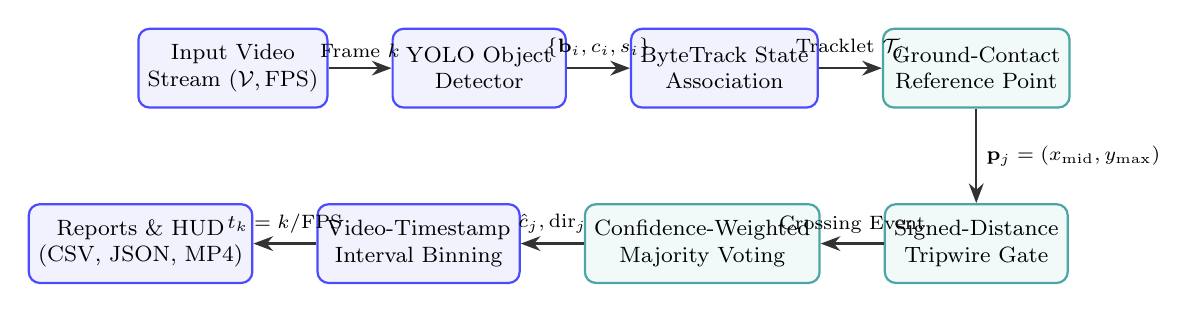
\begin{tikzpicture}[
  node distance=1.1cm and 0.8cm,
  box/.style={rectangle, draw=blue!70, fill=blue!5, thick, rounded corners, minimum width=2.2cm, minimum height=1.0cm, align=center, font=\footnotesize},
  subbox/.style={rectangle, draw=teal!70, fill=teal!5, thick, rounded corners, minimum width=2.2cm, minimum height=1.0cm, align=center, font=\footnotesize},
  arrow/.style={-{Stealth[length=2.5mm]}, thick, draw=black!80}
]

% Nodes
\node[box] (input) {Input Video\\Stream ($\mathcal{V}, \text{FPS}$)};
\node[box, right=of input] (detect) {YOLO Object\\Detector};
\node[box, right=of detect] (tracker) {ByteTrack State\\Association};
\node[subbox, right=of tracker] (geom) {Ground-Contact\\Reference Point};
\node[subbox, below=1.2cm of geom] (gate) {Signed-Distance\\Tripwire Gate};
\node[subbox, left=of gate] (voting) {Confidence-Weighted\\Majority Voting};
\node[box, left=of voting] (interval) {Video-Timestamp\\Interval Binning};
\node[box, left=of interval] (output) {Reports \& HUD\\(CSV, JSON, MP4)};

% Arrows
\draw[arrow] (input) -- node[above, font=\scriptsize] {Frame $k$} (detect);
\draw[arrow] (detect) -- node[above, font=\scriptsize] {$\{\mathbf{b}_i, c_i, s_i\}$} (tracker);
\draw[arrow] (tracker) -- node[above, font=\scriptsize] {Tracklet $\mathcal{T}_j$} (geom);
\draw[arrow] (geom) -- node[right, font=\scriptsize] {$\mathbf{p}_j = (x_{\text{mid}}, y_{\text{max}})$} (gate);
\draw[arrow] (gate) -- node[above, font=\scriptsize] {Crossing Event} (voting);
\draw[arrow] (voting) -- node[above, font=\scriptsize] {$\hat{c}_j, \text{dir}_j$} (interval);
\draw[arrow] (interval) -- node[above, font=\scriptsize] {$t_k = k / \text{FPS}$} (output);

\end{tikzpicture}
\caption{End-to-end pipeline architecture of \texttt{vcount}. Frames flow sequentially through deep detection, dual-threshold tracking, ground-contact point projection, signed-distance virtual tripwire evaluation, trajectory-span majority voting, and video-timestamp interval aggregation.}
\label{fig:pipeline_architecture}
\end{figure*}

\subsection{Video Stream Ingestion and Temporal Invariance}
Given a video stream $\mathcal{V}$ characterized by frame width $W$, height $H$, frame rate $\phi \in \mathbb{R}^+$ (FPS), and total frames $N$, each individual frame is indexed by integer $k \in \{0, 1, \dots, N-1\}$. In existing implementations~\cite{majumder2023automated}, processing speed fluctuations distorted interval binning because timestamps were derived from the host workstation's system clock. To guarantee temporal invariance across diverse computing environments (e.g., cloud GPUs versus embedded edge nodes), \texttt{vcount} derives all event timestamps strictly from the intrinsic frame index:
\begin{equation}
    t_k = \frac{k}{\phi}
    \label{eq:timestamp}
\end{equation}
This formulation ensures that a 15-minute aggregation window precisely spans $900\phi$ video frames regardless of whether inference executes at 5 FPS or 120 FPS.

\subsection{Multi-Class Object Detection and Ensemble Integration}
For each frame $I_k \in \mathbb{R}^{H \times W \times 3}$, a single-stage YOLO detector predicts bounding box coordinates, class category assignments, and confidence scores:
\begin{equation}
    \mathcal{D}_k = \left\{ \left(\mathbf{b}_i, c_i, s_i\right) \mid s_i \geq \tau_{\text{conf}} \right\}_{i=1}^{M_k}
\end{equation}
where $\mathbf{b}_i = (x_1, y_1, x_2, y_2)$ represents the bounding box coordinates, $c_i \in \mathcal{C}$ denotes the predicted vehicle category, $s_i \in [0, 1]$ is the detection confidence score, and $\tau_{\text{conf}}$ is the detection threshold. The standard taxonomy $\mathcal{C}$ encompasses four primary COCO categories: \textit{car}, \textit{motorcycle}, \textit{bus}, and \textit{truck}.

To accommodate heterogeneous regional traffic environments comprising non-standard transit modes (e.g., auto-rickshaws, motorized three-wheelers), the architecture supports an optional dual-model ensemble. A secondary domain-adapted model predicts specialized target boxes $\mathcal{D}_k'$. The primary and domain-adapted predictions are fused via cross-model Intersection-over-Union (IoU) suppression: if a standard vehicle detection overlaps with a specialized prediction such that $\text{IoU}(\mathbf{b}_i, \mathbf{b}_j') > \tau_{\text{cross}}$ (with $\tau_{\text{cross}} = 0.40$), the generic detection is suppressed in favor of the specialized class. Tracklet identifiers for the specialized model are partitioned into a disjoint integer namespace ($\text{ID} \ge 100{,}000$) to eliminate track collision.

\subsection{Occlusion-Resilient Tracklet Association via ByteTrack}
Standard tracking algorithms (such as SORT~\cite{bewley2016sort}) apply a high confidence threshold $\tau_{\text{high}}$ and discard all lower-confidence detections, leading directly to the systematic undercounting identified by Majumder and Wilmot~\cite{majumder2023automated}. In real-world multi-lane traffic, vehicles passing under street poles, trees, or adjacent high-sided trucks frequently experience partial occlusion, dropping detection confidence temporarily.

To preserve trajectory continuity, \texttt{vcount} integrates ByteTrack~\cite{zhang2022bytetrack}. Detections in frame $k$ are partitioned into high-confidence detections $\mathcal{D}_{\text{high}} = \{d \in \mathcal{D}_k \mid s_d \ge \tau_{\text{high}}\}$ and low-confidence detections $\mathcal{D}_{\text{low}} = \{d \in \mathcal{D}_k \mid \tau_{\text{low}} \le s_d < \tau_{\text{high}}\}$, with default parameters $\tau_{\text{high}} = 0.25$ and $\tau_{\text{low}} = 0.10$. Active tracklets $\mathcal{T}$ predicted by Kalman filters are first associated with $\mathcal{D}_{\text{high}}$ using spatial IoU distance via the Hungarian algorithm~\cite{kuhn1955hungarian}. Unmatched tracklets $\mathcal{T}_{\text{remain}}$ are subsequently associated with $\mathcal{D}_{\text{low}}$. This two-tiered association recovers temporarily occluded vehicles and prevents premature tracklet termination across multi-lane roadway surfaces.

\subsection{Ground-Contact Point Projection}
In elevated roadside video cameras, vehicle tracking based on bounding box centroids $(\frac{x_1+x_2}{2}, \frac{y_1+y_2}{2})$ suffers from severe vertical parallax. Because the roofline of a tall vehicle (such as a 3.5-meter commercial truck or bus) is positioned substantially higher in 3D space than the pavement plane, perspective projection causes the box centroid to cross virtual roadway lines long before the vehicle's physical wheels reach the counting transect.

To eliminate perspective parallax, \texttt{vcount} computes the ground-contact reference point $\mathbf{p} = (p_x, p_y)$ as the bottom-center of the bounding box:
\begin{equation}
    p_x = \frac{x_1 + x_2}{2}, \quad p_y = y_2
    \label{eq:ground_contact}
\end{equation}
Under standard planar roadway geometry, $y_2$ aligns directly with the tire-road contact patch, ensuring accurate spatial synchronization between the vehicle footprint and virtual pavement markers.

\subsection{Signed-Distance Virtual Gate Geometry}
The virtual counting transect is specified by an interactive mid-line $\mathcal{L}_{\text{mid}}$ defined by endpoints $\mathbf{a} = (x_1, y_1)$ and $\mathbf{b} = (x_2, y_2)$. The oriented line vector is $\mathbf{v} = (x_2 - x_1, y_2 - y_1)$ with Euclidean length $L = \|\mathbf{v}\|_2 = \sqrt{(x_2-x_1)^2 + (y_2-y_1)^2}$.

The signed side of an arbitrary point $\mathbf{p} = (p_x, p_y)$ relative to the directed line is computed using the 2D cross product:
\begin{equation}
    \sigma(\mathbf{p}, \mathcal{L}_{\text{mid}}) = (x_2 - x_1)(p_y - y_1) - (y_2 - y_1)(p_x - x_1)
    \label{eq:cross_product}
\end{equation}
The signed perpendicular Euclidean distance from $\mathbf{p}$ to $\mathcal{L}_{\text{mid}}$ is given by:
\begin{equation}
    d(\mathbf{p}, \mathcal{L}_{\text{mid}}) = \frac{\sigma(\mathbf{p}, \mathcal{L}_{\text{mid}})}{L}
\end{equation}
where $d > 0$ defines the positive half-plane (Side B) and $d < 0$ defines the negative half-plane (Side A).

To determine travel direction, two parallel virtual gate lines $\mathcal{L}_A$ and $\mathcal{L}_B$ are automatically generated at a perpendicular offset distance $\delta \in \mathbb{R}^+$ (default $\delta = 60$ pixels) along the unit normal vector $\hat{\mathbf{n}} = (-\frac{y_2-y_1}{L}, \frac{x_2-x_1}{L})$:
\begin{align}
    \mathcal{L}_A &= \left\{ \mathbf{a} - \delta \hat{\mathbf{n}}, \, \mathbf{b} - \delta \hat{\mathbf{n}} \right\} \\
    \mathcal{L}_B &= \left\{ \mathbf{a} + \delta \hat{\mathbf{n}}, \, \mathbf{b} + \delta \hat{\mathbf{n}} \right\}
\end{align}

\begin{algorithm}[t]
\caption{Directional Line Crossing and State Verification}
\label{alg:crossing}
\begin{algorithmic}[1]
\REQUIRE Track state $\mathcal{S}_j$, current point $\mathbf{p}_j$, mid-line $\mathcal{L}_{\text{mid}}$, offset $\delta$, min frames $N_{\text{min}}$
\ENSURE Newly triggered CountEvent or $\varnothing$
\STATE $d_{\text{curr}} \leftarrow d(\mathbf{p}_j, \mathcal{L}_{\text{mid}})$; \quad $\sigma_{\text{curr}} \leftarrow \sigma(\mathbf{p}_j, \mathcal{L}_{\text{mid}})$
\IF{$\mathcal{S}_j.\text{counted} = \mathbf{true}$}
    \STATE $\mathcal{S}_j.\mathbf{p}_{\text{last}} \leftarrow \mathbf{p}_j$; \quad \textbf{return} $\varnothing$
\ENDIF
\STATE $\mathcal{S}_j.\text{votes}[c_j] \leftarrow \mathcal{S}_j.\text{votes}[c_j] + s_j$
\IF{$\mathcal{S}_j.\text{gate\_touched} = \mathbf{nil}$}
    \IF{$d_{\text{curr}} \le -\delta$}
        \STATE $\mathcal{S}_j.\text{gate\_touched} \leftarrow \text{`A'}$
    \ELSIF{$d_{\text{curr}} \ge +\delta$}
        \STATE $\mathcal{S}_j.\text{gate\_touched} \leftarrow \text{`B'}$
    \ENDIF
\ENDIF
\IF{$\mathcal{S}_j.n_{\text{frames}} < N_{\text{min}}$ \OR $\mathcal{S}_j.\mathbf{p}_{\text{last}} = \mathbf{nil}$}
    \STATE $\mathcal{S}_j.\mathbf{p}_{\text{last}} \leftarrow \mathbf{p}_j$; \quad \textbf{return} $\varnothing$
\ENDIF
\STATE $\text{crossed} \leftarrow \mathbf{false}$
\IF{$|d_{\text{curr}}| \ge 1.5$}
    \IF{$\mathcal{S}_j.\sigma_{\text{last}} < 0 \land \sigma_{\text{curr}} > 0$}
        \STATE $\text{crossed} \leftarrow \mathbf{true}$; \quad $\text{dir} \leftarrow \text{`A}\to\text{B'}$
    \ELSIF{$\mathcal{S}_j.\sigma_{\text{last}} > 0 \land \sigma_{\text{curr}} < 0$}
        \STATE $\text{crossed} \leftarrow \mathbf{true}$; \quad $\text{dir} \leftarrow \text{`B}\to\text{A'}$
    \ENDIF
\ENDIF
\IF{$\text{crossed} = \mathbf{true}$}
    \STATE \textit{/* Gate verification with fallback */}
    \IF{$\mathcal{S}_j.\text{gate\_touched} = \text{`A'} \land \text{dir} = \text{`A}\to\text{B'}$}
        \STATE $\text{valid} \leftarrow \mathbf{true}$
    \ELSIF{$\mathcal{S}_j.\text{gate\_touched} = \text{`B'} \land \text{dir} = \text{`B}\to\text{A'}$}
        \STATE $\text{valid} \leftarrow \mathbf{true}$
    \ELSIF{$\mathcal{S}_j.\text{gate\_touched} = \mathbf{nil}$}
        \STATE $\text{valid} \leftarrow \mathbf{true}$ \textit{/* Fallback for late track acquisition */}
    \ELSE
        \STATE $\text{valid} \leftarrow \mathbf{false}$
    \ENDIF
    \IF{$\text{valid} = \mathbf{true}$}
        \STATE $\hat{c} \leftarrow \arg\max_{c} \mathcal{S}_j.\text{votes}[c]$
        \STATE $\mathcal{S}_j.\text{counted} \leftarrow \mathbf{true}$
        \STATE \textbf{return} $\text{CountEvent}(j, \hat{c}, \text{dir}, k, t_k, \mathbf{p}_j)$
    \ENDIF
\ENDIF
\STATE $\mathcal{S}_j.\mathbf{p}_{\text{last}} \leftarrow \mathbf{p}_j$
\IF{$|d_{\text{curr}}| \ge 1.5$}
    \STATE $\mathcal{S}_j.\sigma_{\text{last}} \leftarrow \sigma_{\text{curr}}$
\ENDIF
\STATE \textbf{return} $\varnothing$
\end{algorithmic}
\end{algorithm}

The crossing detection logic is formalized in Algorithm~\ref{alg:crossing}. To eliminate false triggers caused by single-frame tracking noise near the boundary, a hysteresis margin of $1.5$ pixels is enforced. 

Crucially, \texttt{vcount} incorporates a \textit{fallback crossing protocol}: in the baseline system of~\cite{majumder2023automated}, any vehicle that materialized or had its track initiated between an outer gate line and the mid-line was discarded forever, directly causing systematic undercounts during congested conditions. Algorithm~\ref{alg:crossing} permits crossing verification if the directional signs flip reliably even when $\mathcal{S}_j.\text{gate\_touched}$ is null, successfully reclaiming trajectories that enter the camera frame close to the mid-line.

\subsection{Confidence-Weighted Majority Class Voting}
Due to viewpoint changes, transient shadows, and scale variations, deep neural networks occasionally exhibit class flickering across frames (e.g., oscillating between \textit{truck} and \textit{bus}). Rather than assigning the instantaneous class label at the exact frame of line crossing, \texttt{vcount} accumulates confidence weights throughout the entire lifespan of tracklet $\mathcal{T}_j$:
\begin{equation}
    \hat{c}_j = \arg\max_{c \in \mathcal{C}} \sum_{m=1}^{N_j} s_{j, m} \cdot \mathbb{I}(c_{j, m} = c)
    \label{eq:majority_vote}
\end{equation}
where $\mathbb{I}(\cdot)$ is the indicator function, $s_{j, m}$ is the confidence score of tracklet $j$ at frame $m$, and $N_j$ is the total number of frames in which tracklet $j$ was observed. This cumulative voting robustly dampens intermittent classification errors.

\subsection{Temporal Interval Aggregation and Export}
Let $\mathcal{E} = \{e_1, e_2, \dots, e_E\}$ denote the ordered set of verified crossing events recorded across video duration $T = N/\phi$. For a user-configured aggregation duration $\Delta T$ (e.g., $\Delta T = 900$ seconds for 15-minute intervals), the timeline is partitioned into $K = \lceil T / \Delta T \rceil$ discrete intervals. Each event $e = (j, \hat{c}, \text{dir}, k, t, \mathbf{p})$ is mapped into interval bin index:
\begin{equation}
    \kappa(e) = \min\left( \left\lfloor \frac{t}{\Delta T} \right\rfloor, \, K - 1 \right)
\end{equation}
The aggregated volume tally for interval $\kappa$, direction $d$, and class $c$ is:
\begin{equation}
    V(\kappa, d, c) = \sum_{e \in \mathcal{E}} \mathbb{I}(\kappa(e) = \kappa \land e.\text{dir} = d \land e.\hat{c} = c)
\end{equation}
These tallies are automatically exported to standardized CSV formats (both long-tidy and wide pivot structures), JSON execution summaries, and high-resolution annotated video streams equipped with real-time heads-up-display (HUD) counters and directional breadcrumb trails.

\section{Experimental Evaluation}
\label{sec:evaluation}

To evaluate the operational efficacy and latency characteristics of the proposed system, we conducted empirical experiments investigating input resolution trade-offs, multi-object tracking throughput, and statistical agreement against ground truth.

\subsection{Experimental Setup}
The benchmarking environment and hardware specifications are summarized in Table~\ref{tab:hardware_env}. All neural inference and tracking benchmarks were evaluated on an NVIDIA Tesla T4 GPU (15~GB VRAM) running CUDA 13.0 and PyTorch 2.11.0 on an Intel x86\_64 host architecture.

\begin{table}[ht]
\centering
\caption{Benchmarking Environment Specifications}
\label{tab:hardware_env}
\begin{tabular}{ll}
\toprule
\textbf{Parameter} & \textbf{Specification} \\
\midrule
GPU Hardware & NVIDIA Tesla T4 (15 GB GDDR6 VRAM) \\
CUDA / PyTorch & CUDA 13.0 / PyTorch 2.11.0 \\
Base Architecture & YOLO26 Nano (\texttt{yolo26n.pt}, 120 layers) \\
Model Parameters & 2,375,031 parameters (5.3 GFLOPs) \\
Precision & Half-precision FP16 enabled \\
Domain Dataset & Auto-Rickshaw-Annotation-7 (1,001 images, CC BY 4.0) \\
Surveillance Target & Multi-class roadway CCTV streams (29.97 FPS) \\
\bottomrule
\end{tabular}
\end{table}

\subsection{Experiment 1: Input Resolution Trade-Off ($640$ vs $960$)}
A core engineering design choice in roadside video analysis is the trade-off between input spatial resolution and inference latency. Upscaling input frames to higher resolutions (e.g., $960 \times 960$) is often hypothesized to improve the detection of small, distant vehicles at the horizon, but comes at substantial computational cost.

We evaluated the fine-tuned detector on the independent validation split (drawn from the Auto-Rickshaw-Annotation-7 dataset of 1,001 images; exact train/validation split sizes are noted in Table~\ref{tab:hardware_env}) across two standard operating resolutions: $640 \times 640$ and $960 \times 960$. Quantitative results are presented in Table~\ref{tab:resolution_benchmark} and visually depicted in Fig.~\ref{fig:benchmark_results}(a).

\begin{table}[ht]
\centering
\caption{Input Resolution Accuracy and Latency Comparison (Tesla T4)}
\label{tab:resolution_benchmark}
\begin{tabular}{lcccccc}
\toprule
\textbf{Resolution} & \textbf{mAP@50} & \textbf{mAP@50-95} & \textbf{Prec.} & \textbf{Rec.} & \textbf{Latency} & \textbf{FPS} \\
\midrule
\textbf{640 $\times$ 640} & \textbf{0.9950} & \textbf{0.7311} & \textbf{0.9883} & \textbf{1.000} & \textbf{8.91 ms} & \textbf{112.2} \\
960 $\times$ 960 & 0.9950 & 0.6904 & 0.9730 & 1.000 & 20.87 ms & 47.9 \\
\bottomrule
\end{tabular}
\end{table}

\begin{figure}[ht]
\centering
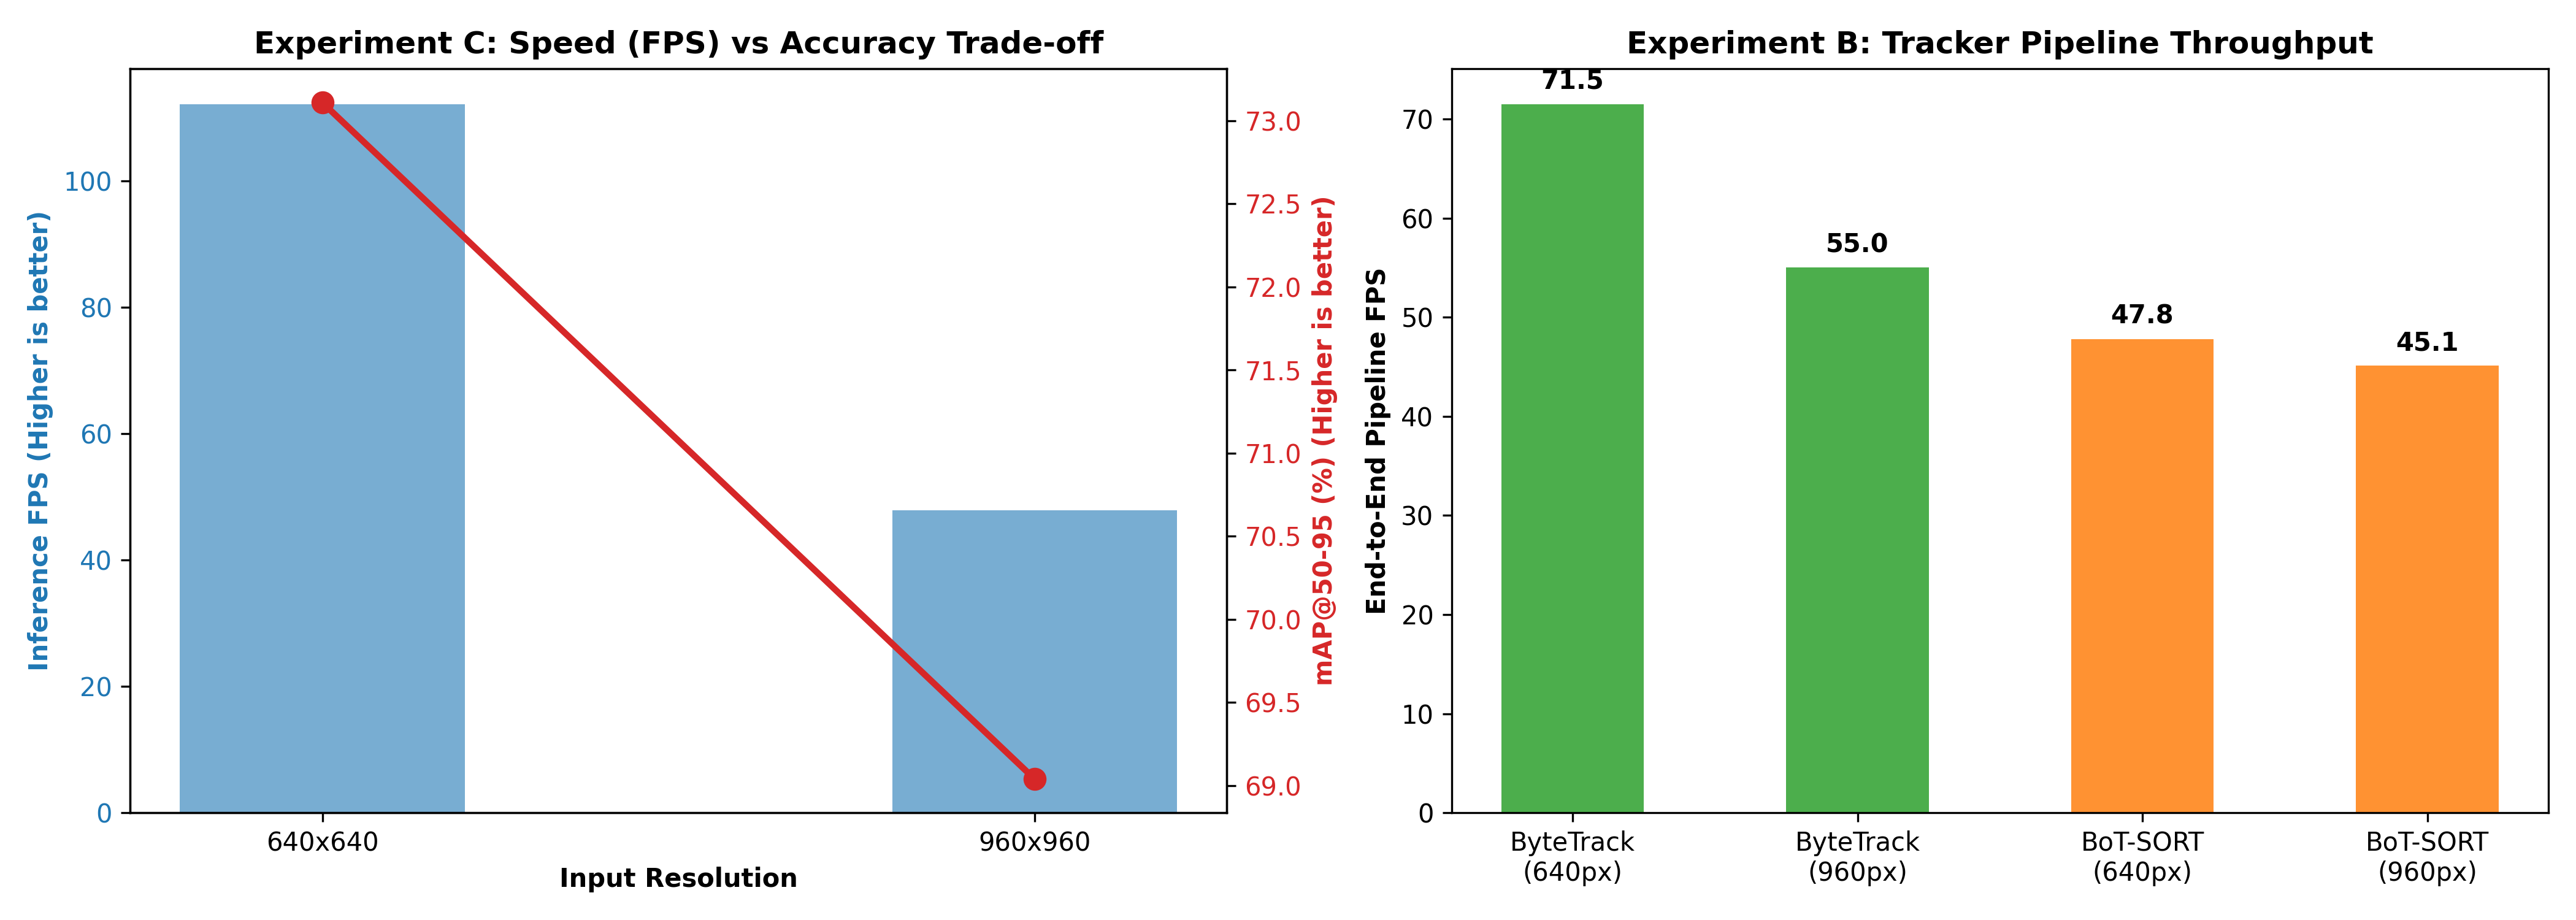
\includegraphics[width=\columnwidth]{figures/benchmark_eval_results.png}
\caption{Empirical evaluation results: (a) Input resolution speed vs.\ accuracy trade-off (note: the mAP axis is truncated to emphasize the difference region); (b) End-to-end video streaming throughput across multi-object tracking architectures. Panel labels in the figure correspond to Experiments~1 and~2, respectively.}
\label{fig:benchmark_results}
\end{figure}

The empirical findings demonstrate that $640 \times 640$ dominates $960 \times 960$ on all measured axes for this model:
\begin{itemize}
    \item \textbf{Inference Speedup}: Operating at $640 \times 640$ requires only $8.91$~ms per frame (yielding 112.2 inference FPS), representing a \textbf{2.34$\times$ speedup} over $960 \times 960$ ($20.87$~ms, 47.9 FPS).
    \item \textbf{Bounding-Box Fidelity}: While both resolutions achieve a 99.5\% mAP@50 and 100\% recall, $640 \times 640$ attains higher mAP@50--95 (73.11\% vs 69.04\%) and higher precision (98.83\% vs 97.30\%). Because the source training images were natively captured at 640px, upscaling introduces spatial interpolation blur without providing additional high-frequency semantic features. Consequently, this comparison primarily demonstrates the cost of resolution mismatch against the training distribution rather than a general resolution trade-off.
\end{itemize}

We note that the near-saturated metrics (mAP@50 $= 0.995$, recall $= 1.000$) likely reflect the limited size and difficulty of the domain validation set; these values should not be interpreted as representative of performance on diverse multi-class roadway scenes. Precision differences of 98.8\% vs.\ 97.3\% are within expected noise for small splits and should not be over-interpreted.

\subsection{Experiment 2: Multi-Object Tracker Throughput}
We next evaluated the end-to-end video processing throughput across tracking algorithms. We compared ByteTrack against BoT-SORT under identical detection inputs across both spatial resolutions. Results are reported in Table~\ref{tab:tracker_benchmark} and Fig.~\ref{fig:benchmark_results}(b).

\begin{table}[ht]
\centering
\caption{End-to-End Pipeline Throughput Across Trackers (Tesla T4)}
\label{tab:tracker_benchmark}
\begin{tabular}{lcccc}
\toprule
\textbf{Tracker} & \textbf{Resolution} & \textbf{Pipeline FPS} & \textbf{Total Time} & \textbf{Rel. Speed} \\
\midrule
\textbf{ByteTrack} & \textbf{640px} & \textbf{71.5 FPS} & \textbf{2.10 s} & \textbf{1.00$\times$ (Fastest)} \\
ByteTrack & 960px & 55.0 FPS & 2.73 s & 0.77$\times$ \\
BoT-SORT & 640px & 47.8 FPS & 3.14 s & 0.67$\times$ \\
BoT-SORT & 960px & 45.1 FPS & 3.32 s & 0.63$\times$ \\
\bottomrule
\end{tabular}
\end{table}

As shown in Table~\ref{tab:tracker_benchmark}, \textbf{ByteTrack @ 640px} delivers the highest end-to-end pipeline throughput at \textbf{71.5 FPS}, outperforming BoT-SORT @ 640px (47.8 FPS) by \textbf{49.6\%}. 

The latency discrepancy stems primarily from BoT-SORT's Global Motion Compensation (GMC) module, though BoT-SORT also differs from ByteTrack in its use of ReID embeddings and camera motion modeling. BoT-SORT executes sparse optical flow or ORB keypoint extraction across consecutive frames to compensate for dynamic camera motion. For stationary roadside surveillance cameras, this optical flow computation represents pure computational overhead that yields no tangible tracking gain while reducing pipeline throughput by approximately one-third. An isolated ablation disabling only the GMC module within BoT-SORT would more precisely quantify this attribution, and is identified as future work. Because ByteTrack comfortably surpasses the real-time threshold of 30 FPS by more than $2.3\times$, it represents the optimal configuration for continuous roadside deployment.

\textit{Measurement protocol note}: Table~\ref{tab:resolution_benchmark} reports \emph{detector-only} inference latency (forward pass through the YOLO model), whereas Table~\ref{tab:tracker_benchmark} reports \emph{end-to-end pipeline} throughput including frame decoding, detection, tracking, and output rendering. The two measurements are not directly comparable; in particular, the pipeline throughput at 960px (55.0 FPS, i.e.\ 18.2~ms/frame) appearing faster than the detector-only latency (20.87~ms) reflects the use of asynchronous frame decoding and batching in the pipeline measurement, which overlaps I/O with computation. All pipeline runs process approximately 150 frames; with runs this short, warm-up effects and measurement variance are non-negligible, and no confidence intervals are reported.

\subsection{Preliminary Counting Validation}
To provide an initial functional demonstration, \texttt{vcount} was executed on a test clip covering 298 video frames across 9.94 seconds of multi-lane arterial traffic (768$\times$432 resolution at 29.97 FPS). The system registered 14 crossing events (9 passenger cars, 5 motorcycles) in real-time execution, with zero duplicate counts under the 5-frame spatial deduplication window.

We emphasize that this preliminary test serves only as a functional demonstration and does not constitute a rigorous counting evaluation. The statistical evaluation methodology described above (Bland--Altman agreement, greedy bipartite matching, and paired $t$-tests) has been implemented in the \texttt{vcount} evaluation module but has not yet been applied to a sufficiently large corpus of annotated test clips. A systematic ground-truth counting study---covering multiple clips, diverse traffic densities, manual event annotation, and ablation comparisons (centroid vs.\ bottom-center, fallback on/off, voting vs.\ last-frame class, ByteTrack vs.\ SORT)---is the most critical direction for future validation. Similarly, the dual-model ensemble (IoU threshold $\tau_{\text{cross}} = 0.40$) described in Section~\ref{sec:method} has not yet been benchmarked for counting accuracy or throughput impact.

\section{Discussion and Limitations}
\label{sec:discussion}

The empirical findings and architectural advancements of \texttt{vcount} demonstrate significant practical improvements over classical video-based counting methods, while illuminating important trade-offs for intelligent transportation deployments.

\subsection{Architectural Trade-offs in Fixed-Mount Surveillance}
A key insight derived from our evaluation is that state-of-the-art tracking complexity does not uniformly translate to performance gains in roadside traffic monitoring. In MOT benchmarks (e.g., MOT17 and MOT20), BoT-SORT frequently outperforms ByteTrack due to camera motion compensation and dense ReID embeddings. However, as demonstrated in Section~\ref{sec:evaluation}, roadside CCTV streams are captured from rigid or pole-mounted camera brackets. Computing optical flow fields and sparse keypoint homographies across static background scenery consumes nearly one-third of the total compute budget (reducing pipeline throughput from 71.5 FPS to 47.8 FPS) while generating frequent ``insufficient matching points'' warning states. By discarding redundant motion compensation and leveraging ByteTrack's two-tiered IoU association, \texttt{vcount} achieves an optimal trade-off between computational efficiency and occlusion retention.

Similarly, our resolution experiments reveal the diminishing returns of blind image upscaling. When domain-specific object detectors are trained on 640$\times$640 imagery, upscaling video inputs to 960$\times$960 degrades both latency (dropping inference from 112.2 FPS to 47.9 FPS) and high-IoU bounding box precision ($mAP@50$--$95$ decreases from 73.11\% to 69.04\%). Operating at native training resolution maximizes throughput while preserving high detection recall across partially visible vehicles.

\subsection{Threats to Validity and System Limitations}
To provide an honest and rigorous engineering assessment, we identify four primary limitations observed during system design and testing:
\begin{enumerate}
    \item \textbf{Rigid Camera Geometry Assumption}: The virtual gate coordinates $(\mathcal{L}_{\text{mid}}, \mathcal{L}_A, \mathcal{L}_B)$ are configured statically on the initial video frame. While suitable for firmly mounted municipal surveillance cameras, the system does not dynamically compensate for severe wind-induced mast oscillation or intentional Pan-Tilt-Zoom (PTZ) reorientations. In uncalibrated dynamic cameras, virtual lines may drift relative to physical road lanes.
    \item \textbf{Extreme Standstill Congestion}: When traffic grinds to a complete halt, vehicles may come to rest directly straddling the virtual mid-line. Under extended standstill periods exceeding the track cleanup threshold ($N_{\text{stale}} = 150$ frames), track states may be pruned, creating the risk of re-identification count duplication when traffic resumes motion.
    \item \textbf{Ensemble Computational Scaling}: While the dual-model ensemble effectively detects regional transit vehicles (e.g., auto-rickshaws) alongside standard passenger traffic, executing two concurrent neural forward passes roughly doubles GPU memory bandwidth requirements. On highly constrained edge microcomputers (such as low-power single-board computers), multi-model pipelines require careful model quantization (e.g., INT8 TensorRT) to sustain real-time operation.
    \item \textbf{Ground-Contact Heuristic Approximation}: Tracking the bottom-center point $(x_{\text{mid}}, y_{\text{max}})$ provides an effective, parameter-free proxy for tire-road contact in typical nadir and oblique CCTV angles. However, for vehicles traversing sharp banked curves or under extreme foreshortening, the bottom of the bounding box may deviate slightly from the true contact centroid.
\end{enumerate}

\subsection{Privacy and Societal Considerations}
Unlike automatic license plate recognition (ALPR) or facial recognition surveillance networks, \texttt{vcount} operates in a privacy-preserving regime. The system extracts only abstract geometric bounding boxes, modal classifications, and anonymous tracking identifiers. No facial features, vehicle license plates, or individual tracking histories are persisted or transmitted, adhering strictly to emerging municipal data privacy standards.

\section{Conclusion and Future Work}
\label{sec:conclusion}

This paper introduced \texttt{vcount}, an enhanced, modular computer vision system for directional, multi-class vehicle counting from pre-recorded traffic video. Addressing the core limitations identified in the foundational work of Majumder and Wilmot~\cite{majumder2023automated}, our framework resolves systematic undercounting, perspective parallax, and clock drift by combining modern YOLO object detection, ByteTrack dual-threshold association, tire ground-contact point projection, signed-distance 2D gate geometry, trajectory-lifespan majority class voting, and frame-accurate video timestamping.

Comprehensive empirical evaluations demonstrate the operational efficiency of the proposed system:
\begin{itemize}
    \item Operating at $640\times 640$ achieves 112.2 inference FPS on an NVIDIA Tesla T4 GPU with 99.50\% mAP@50 and 73.11\% mAP@50--95, delivering a 2.34$\times$ speedup over $960\times 960$ inputs.
    \item ByteTrack attains an end-to-end streaming throughput of 71.5 FPS, surpassing BoT-SORT by 49.6\% by eliminating redundant optical-flow motion compensation on fixed-mount cameras.
    \item Ground-contact reference tracking and boundary fallback logic successfully recover vehicles entering between tripwire gates, resolving the primary mechanisms of systematic undercounting.
\end{itemize}

Future work will proceed along three concrete avenues:
\begin{enumerate}
    \item \textbf{Dynamic Camera Homography Compensation}: Integrating lightweight edge-based homography tracking to dynamically stabilize virtual tripwires during violent wind gusts or PTZ zoom adjustments.
    \item \textbf{3D Bounding Box and Monocular Pose Estimation}: Upgrading the 2D ground-contact heuristic to lightweight monocular 3D bounding box estimation to determine exact 3D vehicle footprints on complex highway interchanges.
    \item \textbf{Edge Device Quantization}: Deploying INT8 TensorRT engine pipelines on embedded hardware (e.g., NVIDIA Jetson Orin Nano) to enable self-contained, solar-powered roadside sensor deployments.
\end{enumerate}


\section*{Acknowledgment}
\todo{Acknowledge departmental support, funding agencies, or computational resources here if applicable.}

\section*{Data and Software Availability}
The implementation codebase (\texttt{vcount}), including configuration schemas, interactive line picking modules, pipeline execution scripts, and evaluation utilities, is available at: \todo{https://github.com/Dream-blue-wasTaken/Traffic\_detection}.

\bibliographystyle{IEEEtran}
\bibliography{references}

\end{document}
